\documentclass{book}

\usepackage{xcolor} % define colors
\usepackage{amsthm} % for theorem environments
\usepackage{amssymb} % for math symbols
\usepackage{amsmath} % for advanced math typesetting
\usepackage[margin=1in]{geometry} % set page margins
\usepackage{tikz, tikz-3dplot} % for 2D and 3D graphics
\usepackage[pdfborder={0 0 0}]{hyperref} % for hyperlinks in the document %removed the red box around links
\usepackage{subcaption} % for subcaption

\usepackage{graphicx}


\usepackage{pgfplots}
\pgfplotsset{compat=1.15}


\definecolor{ocre}{RGB}{0,83,166}

\newtheorem{example}{Example}[chapter]
\newtheorem{definition}{Definition}[chapter]
% Non-italic
\theoremstyle{remark}
\newtheorem*{solution}{Solution}
\newtheorem*{remark}{Remark}

%Added some common sets
\newcommand{\N}{\mathbb{N}}
\newcommand{\Z}{\mathbb{Z}}
\newcommand{\Q}{\mathbb{Q}}
\newcommand{\R}{\mathbb{R}}
\newcommand{\C}{\mathbb{C}}


\begin{document}

\frontmatter
\title{\sffamily\Huge\color{ocre} Multivariable Calculus}
\author{\sffamily Department of Mathematics\\\sffamily Hong Kong University of Science and Technology}
\date{\sffamily \today}
\maketitle

\tableofcontents

\mainmatter

\chapter{Vectors and the Geometry of Space}

\section{Three-Dimensional Coordinate Systems}

We would use an ordered tuple of three numbers $(x, y, z)$ to represent a point in three-dimensional space. The three numbers correspond to the distances along the $x$-axis, $y$-axis, and $z$-axis respectively.

Moreover, we can use a vector to represent a point in space. A vector $\mathbf{v}$ can be expressed as:
\[
    \mathbf{v} = \langle x, y, z \rangle = x\mathbf{i} + y\mathbf{j} + z\mathbf{k}
\]
where $\mathbf{i}$, $\mathbf{j}$, and $\mathbf{k}$ are the unit vectors along the $x$-, $y$-, and $z$-axes respectively.

\begin{remark}
    Unit vectors are vectors with a magnitude of 1. They are often used to indicate direction.
\end{remark}

The distance, or norm, of the vector $\mathbf{v}$ from the origin can be calculated using the formula:
\[
    \|\mathbf{v}\|_2 = \|\mathbf{v}\| = \sqrt{x^2 + y^2 + z^2}
\]
This is also known as the Euclidean norm.

As we are used to consider two-dimensional planes, we always consider the following equations as circles in two-dimensional space:
\[
    x^2 + y^2 = r^2
\]
However, in three-dimensional space, this equation represents a cylinder extending infinitely along the $z$-axis. As implicitly, the equation does not restrict the value of $z$. Then the set of points satisfying the equation forms a cylinder.

In two-dimensional case, the set of points satisfying the equation $x^2 + y^2 = r^2$ represents a circle of radius $r$ centered at the origin:
\[
    S^1 = \{ (x, y) \mid x^2 + y^2 = r^2 \}
\]
In three-dimensional case, the set of points satisfying the equation $x^2 + y^2 = r^2$ represents a cylinder of radius $r$ centered along the $z$-axis:
\[
    C = \{ (x, y, z) \mid x^2 + y^2 = r^2, z \in \mathbb{R} \}
\]

So if we want to represent a two-dimensional circle in three-dimensional space, we need to add an additional constraint on $z$. For example, the set of points satisfying the equations $x^2 + y^2 = r^2$ and $z = 0$ represents a circle of radius $r$ in the $xy$-plane:
\[
    S^1 = \{ (x, y, z) \mid x^2 + y^2 = r^2, z = 0 \}
\]

For vector operations, we have:
\begin{itemize}
    \item Vector Addition: $\mathbf{a} + \mathbf{b} = \langle a_1 + b_1, a_2 + b_2, a_3 + b_3 \rangle$
    \item Scalar Multiplication: $c\mathbf{a} = \langle ca_1, ca_2, ca_3 \rangle$
\end{itemize}

Also, we have the dot product and cross product defined as:
\begin{itemize}
    \item Dot Product: $\mathbf{a} \cdot \mathbf{b} = a_1b_1 + a_2b_2 + a_3b_3$
    \item Cross Product: $\mathbf{a} \times \mathbf{b} = \langle a_2b_3 - a_3b_2, a_3b_1 - a_1b_3, a_1b_2 - a_2b_1 \rangle$
\end{itemize}

Moreover, the dot product can also be expressed in terms of the magnitudes of the vectors and the angle $\theta$ between them:
\[
    \mathbf{a} \cdot \mathbf{b} = \|\mathbf{a}\| \|\mathbf{b}\| \cos\theta
\]
and the magnitude of the cross product can be expressed as:
\[
    \|\mathbf{a} \times \mathbf{b}\| = \|\mathbf{a}\| \|\mathbf{b}\| \sin\theta
\]
It represents the area of the parallelogram formed by the two vectors.

If we want to project vector $\mathbf{b}$ onto vector $\mathbf{a}$, we can use the formula:
\[
    \text{proj}_{\mathbf{a}} \mathbf{b} = \left(\frac{\mathbf{a} \cdot \mathbf{b}}{\|\mathbf{a}\|}\right) \frac{\mathbf{a}}{\|\mathbf{a}\|} = \frac{\mathbf{a} \cdot \mathbf{b}}{\|\mathbf{a}\|^2} \mathbf{a}
\]
The scalar projection of $\mathbf{b}$ onto $\mathbf{a}$ is given by:
\[
    \text{comp}_{\mathbf{a}} \mathbf{b} = \|\mathbf{b}\| \cos\theta = \frac{\mathbf{a} \cdot \mathbf{b}}{\|\mathbf{a}\|}
\]

For the cross product, we can use the following determinant form:
\[
    \mathbf{a} \times \mathbf{b} = \begin{vmatrix}
    \mathbf{i} & \mathbf{j} & \mathbf{k} \\
    a_1 & a_2 & a_3 \\
    b_1 & b_2 & b_3
    \end{vmatrix}
\]

\begin{remark}
    The cross product of two vectors results in a vector that is orthogonal (perpendicular) to both original vectors. The direction of the resulting vector is determined by the right-hand rule.
\end{remark}

\section{Lines and Planes}

\subsection{Lines}

To represent a line in three-dimensional space, we can use a point and a direction vector. If we have a point $P_0(x_0, y_0, z_0)$ on the line and a direction vector $\mathbf{v} = \langle v_1, v_2, v_3 \rangle$, then any point $P(x, y, z)$ on the line, the vector $\overrightarrow{P_0P}$ is parallel to $\mathbf{v}$, i.e., $\overrightarrow{P_0P} = t\mathbf{v}$ for some scalar $t$. Then we have the parametric equations of the line as:
\[
    \langle x, y, z \rangle - \langle x_0, y_0, z_0 \rangle = t \langle v_1, v_2, v_3 \rangle
\]
or equivalently,
\[
    \begin{cases}
        x = x_0 + tv_1 \\
        y = y_0 + tv_2 \\
        z = z_0 + tv_3
    \end{cases}
\]
which are called the \emph{parametric equations} of the line. The $t$ is called the \emph{parameter} of the line.

To visualize the parametric equation of a line in 3D, consider Figure \ref{fig:3d_line_parametric} below.
\begin{figure}[ht]
    \centering
    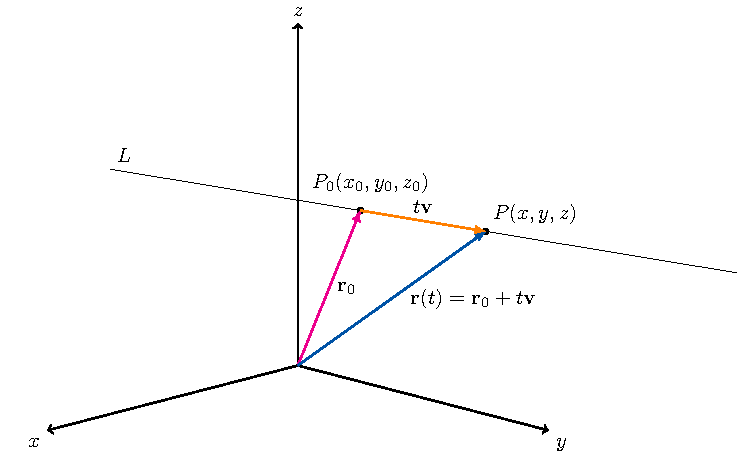
\includegraphics{figures/2d_plane_equation.pdf}
    \caption{Parametric Equation of a Line in 3D}\label{fig:3d_line_parametric}
\end{figure}

From Figure \ref{fig:3d_line_parametric}, we can also write the parametric equations as:
\[
    \mathbf{r}(t) = \overrightarrow{OP_0} + t\mathbf{v}
\]
which is called the \emph{vector form} of the line.

If $\mathbf{v} = \langle v_1, v_2, v_3 \rangle$ where none of $v_1, v_2, v_3$ is zero, we can also express the line in \emph{symmetric form} as:
\[
    \frac{x - x_0}{v_1} = \frac{y - y_0}{v_2} = \frac{z - z_0}{v_3}
\]

\begin{example}
    Find the parametric equations of the line that passes through the points $A(1, 2, 3)$ and $B(4, 5, 6)$. Express the line in vector form, parametric form and symmetric forms.
\end{example}
\begin{solution}
    In order to find the equation of the line, we need 
    \begin{itemize}
        \item A point on the line: $A(1, 2, 3)$;
        \item A direction vector: $\mathbf{v} = \overrightarrow{AB} = \langle 4 - 1, 5 - 2, 6 - 3 \rangle = \langle 3, 3, 3 \rangle$.
    \end{itemize}
    Therefore, the vector form of the line is:
    \[
        \mathbf{r}(t) = \langle 1, 2, 3 \rangle + t \langle 3, 3, 3 \rangle
    \]
    The parametric form of the line is:
    \[
        \begin{cases}
            x = 1 + 3t \\
            y = 2 + 3t \\
            z = 3 + 3t
        \end{cases}
    \]
    The symmetric form of the line is:
    \[
        \frac{x - 1}{3} = \frac{y - 2}{3} = \frac{z - 3}{3}
    \]
\end{solution}

\subsection{Planes}

A plane in three-dimensional space can be defined using a point and a normal vector. If we have a point $P_0(x_0, y_0, z_0)$ on the plane and a normal vector $\mathbf{n} = \langle A, B, C \rangle$, then any point $P(x, y, z)$ on the plane satisfies the condition that the vector $\overrightarrow{P_0P}$ is orthogonal to the normal vector $\mathbf{n}$, i.e., $\mathbf{n} \cdot \overrightarrow{P_0P} = 0$. This leads to the equation of the plane:
\[
    \langle A, B, C \rangle \cdot (\langle x, y, z \rangle - \langle x_0, y_0, z_0 \rangle) = 0
\]
or equivalently,
\[
    A(x - x_0) + B(y - y_0) + C(z - z_0) = 0
\]
which is called the \emph{scalar equation} of the plane. 

Expanding this, we get:
\[
    Ax + By + Cz = Ax_0 + By_0 + Cz_0
\]
or equivalently,
\[
    Ax + By + Cz + D = 0
\]
where $D = -(Ax_0 + By_0 + Cz_0)$ is a constant. It is called a \emph{linear equation} in $x$, $y$ and $z$.

To visualize the equation of a plane in 3D, consider Figure \ref{fig:3d_plane_equation} below.
\begin{figure}[ht]
    \centering
    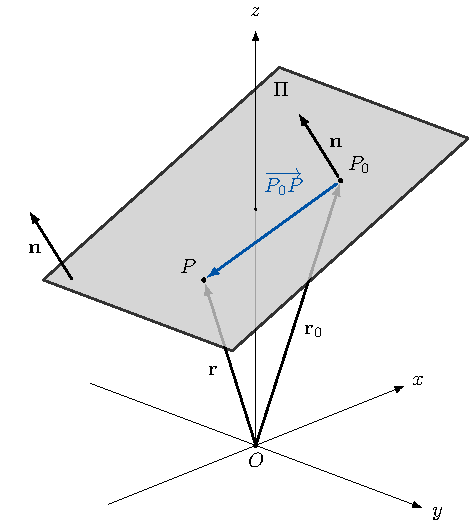
\includegraphics{figures/3d_plane_equation.pdf}
    \caption{Equation of a Plane in 3D}\label{fig:3d_plane_equation}
\end{figure}

In order to find $\mathbf{n}$, we can use the cross product.
\begin{example}
    Find the equation of the plane that passes through the points:
    \[
        A(1, 2, 3), \quad B(4, 5, 6), \quad C(7, 8, 0).
    \]
\end{example}
\begin{solution}
    In order to find the equation of the plane, we need
    \begin{itemize}
        \item A point on the plane: $A(1, 2, 3)$;
        \item A normal vector: $\mathbf{n} = \overrightarrow{AB} \times \overrightarrow{AC}$.
    \end{itemize}
    First, we calculate the vectors $\overrightarrow{AB}$ and $\overrightarrow{AC}$:
    \[
        \begin{split}
            \overrightarrow{AB} &= \langle 4 - 1, 5 - 2, 6 - 3 \rangle = \langle 3, 3, 3 \rangle, \\
            \overrightarrow{AC} &= \langle 7 - 1, 8 - 2, 0 - 3 \rangle = \langle 6, 6, -3 \rangle.
        \end{split}
    \]
    Taking the cross product, we have:
    \[
        \overrightarrow{AB} \times \overrightarrow{AC} = \begin{vmatrix}
        \mathbf{i} & \mathbf{j} & \mathbf{k} \\
        3 & 3 & 3 \\
        6 & 6 & -3
        \end{vmatrix} = \langle 0, 0, -9 \rangle.
    \]
    For simplicity, we can take the normal vector as $\mathbf{n} = \langle 0, 0, 1 \rangle$. Therefore, the equation of the plane is:
    \[
        \begin{split}
            0(x - 1) + 0(y - 2) + 1(z - 3) &= 0 \\
            z - 3 &= 0 \\
            z &= 3.
        \end{split}
    \]
\end{solution}

If we have a point $P_1(x_1, y_1, z_1)$ not on the plane, we can calculate the distance from the point to the plane using the formula:
\[
    \text{Distance} = \frac{\| \mathbf{n} \cdot \mathbf{b} \|}{\| \mathbf{n} \|} = \frac{A(x_1 - x_0) + B(y_1 - y_0) + C(z_1 - z_0)}{\sqrt{A^2 + B^2 + C^2}} = \frac{|A x_1 + B y_1 + C z_1 + D|}{\sqrt{A^2 + B^2 + C^2}}
\]
where $\mathbf{b} = \overrightarrow{P_0P_1} = \langle x_1 - x_0, y_1 - y_0, z_1 - z_0 \rangle$.

\section{Cylinders and Quadric Surfaces}

\subsection{Cylinders}

A cylinder is a surface that consists of all lines that are parallel to a given line and pass through a given curve. The given line is called the \emph{generatrix} of the cylinder, and the given curve is called the \emph{directrix} of the cylinder.

\begin{example}
    Sketch the graph of the surface defined by the equation:
    \[
        z = x^2
    \]
\end{example}
\begin{solution}
    This equation represents a parabolic cylinder. For any fixed value of $y$, the cross-section in the $xz$-plane is a parabola defined by $z = x^2$. The surface extends infinitely along the $y$-axis, forming a cylinder-like shape. Consider the Figure \ref{fig:parabolic_cylinder} below, which illustrates the parabolic cylinder defined by the equation $z = x^2$. If we take cross-sections at different values of $y$, we obtain parabolas that open upwards in the $xz$-plane.
\end{solution}

\begin{figure}[ht]
    \centering
    \tdplotsetmaincoords{70}{120}
	\begin{tikzpicture}[tdplot_main_coords]
		%%% Coordinate axis
		\draw[thick,-latex] (0,0,0) -- (2.5,0,0) node [below left] {\footnotesize$x$};
		\draw[dashed] (0,0,0) -- (-2.5,0,0);
		\draw[thick,-latex] (0,0,0) -- (0,4.5,0) node [right] {\footnotesize$y$};
		\draw[dashed] (0,0,0) -- (0,-2.5,0);
		\draw[thick] (0,0,0.0) -- (0,0,4.0);
		% The curves slicing the surface
		\draw[ocre,thick] plot[domain=-1.75:1.75,smooth,variable=\t] ({\t},{-2.0},{\t*\t});
		\draw[ocre,thick] plot[domain=-1.75:1.75,smooth,variable=\t] ({\t},{4.0},{\t*\t}); 
        \draw[ocre,thick] plot[domain=-1.75:1.75,smooth,variable=\t] ({\t},{0.0},{\t*\t});
		% The surface
		\foreach \y in {-1.99,-1.98,...,-0.01,0.01,0.02,...,3.99}{
			\draw[black!10,thick,opacity=0.2] plot[domain=-1.75:1.75,smooth,variable=\t] ({\t},{\y},{\t*\t}); 
		}
		%
		\node[above right] at (0,2.5,4.125) {$z = x^2$};
		% Last part of the z axis
		\draw[thick,-latex] (0,0,4.0) -- (0,0,4.5) node [above] {\footnotesize$z$};	
	\end{tikzpicture}
    \caption{Parabolic Cylinder of $z = x^2$}\label{fig:parabolic_cylinder}
\end{figure}

\begin{example}
    Sketch the graph of the surface defined by the equation:
    \[
        x^2 + y^2 = 1
    \]
\end{example}
\begin{solution}
    This equation represents a circular cylinder. For any fixed value of $z$, the cross-section in the $xy$-plane is a circle defined by $x^2 + y^2 = 1$. The surface extends infinitely along the $z$-axis, forming a cylinder-like shape. Consider the Figure \ref{fig:circular_cylinder} below, which illustrates the circular cylinder defined by the equation $x^2 + y^2 = 1$. If we take cross-sections at different values of $z$, we obtain circles in the $xy$-plane.
\end{solution}

\begin{figure}[ht]
    \centering
    \tdplotsetmaincoords{70}{120}
    \begin{tikzpicture}[tdplot_main_coords]
		%%% Coordinate axis
		\draw[thick,-latex] (0,0,0) -- (2.5,0,0) node [below left] {\footnotesize$x$};
		\draw[dashed] (0,0,0) -- (-2.5,0,0);
		\draw[thick,-latex] (0,0,0) -- (0,2.5,0) node [right] {\footnotesize$y$};
		\draw[dashed] (0,0,0) -- (0,-2.5,0);
		\draw[thick] (0,0,0.0) -- (0,0,4.0);
		% The curves slicing the surface
		\draw[ocre,thick,opacity=0.5] (0,0,0) circle (1.0); 
		% The surface
		\foreach \z in {0.01,0.02,...,3.99}{
			\draw[black!10,thick,opacity=0.2] (0,0,\z) circle (1.0); 
		}
		% The curves slicing the surface
		\draw[ocre,thick,opacity=0.5] (0,0,4) circle (1.0);
		%

		\node[right] at (0,1,4) {$x^2 + y^2 = 1$};
		% Last part of the z axis
		\draw[thick,-latex] (0,0,4.0) -- (0,0,4.5) node [above] {\footnotesize$z$};	
    \end{tikzpicture}
    \caption{Circular Cylinder of $x^2 + y^2 = 1$}\label{fig:circular_cylinder}
\end{figure}

\subsection{Quadric Surfaces}
A quadric surface is a surface in three-dimensional space defined by a second-degree polynomial equation in three variables $x$, $y$, and $z$. The general form of a quadric surface equation is:
\[
    Ax^2 + By^2 + Cz^2 + Dxy + Eyz + Fxz + Gx + Hy + Iz + J = 0.
\]
By simple translation or rotations, it can be brought into one of the following forms:
\[
    Ax^2 + By^2 + Cz^2 + J = 0, \quad Ax^2 + By^2 + Iz = 0
\]

There are 6 kinds of quadric surfaces, as shown below:
\begin{figure}[ht]

\centering

\begin{subfigure}{0.3\textwidth}
    \centering
    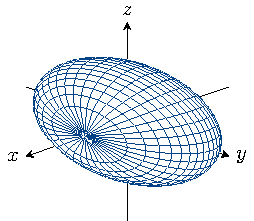
\includegraphics{figures/ellipsoid.pdf}
    \caption{Ellipsoid}
\end{subfigure}
\begin{subfigure}{0.3\textwidth}
    \centering
    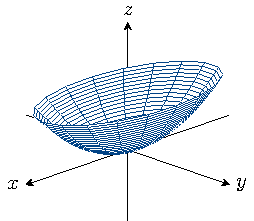
\includegraphics{figures/elliptic_paraboloid.pdf}
    \caption{Elliptic Paraboloid}
\end{subfigure}
\begin{subfigure}{0.3\textwidth}
    \centering
    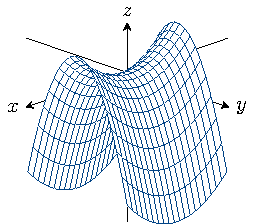
\includegraphics{figures/hyperbolic_paraboloid.pdf}
    \caption{Hyperbolic Paraboloid}
\end{subfigure}
\begin{subfigure}{0.3\textwidth}
    \centering
    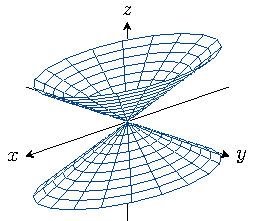
\includegraphics{figures/cone.pdf}
    \caption{Cone}
\end{subfigure}
\begin{subfigure}{0.3\textwidth}
    \centering
    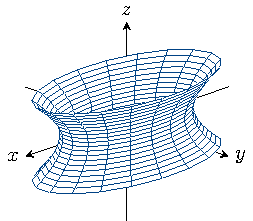
\includegraphics{figures/hyperboloid_of_one_sheet.pdf}
    \caption{Hyperboloid of One Sheet}
\end{subfigure}
\begin{subfigure}{0.3\textwidth}
    \centering
    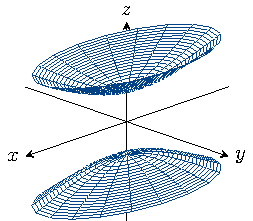
\includegraphics{figures/hyperboloid_of_two_sheets.pdf}
    \caption{Hyperboloid of Two Sheets}
\end{subfigure}

\end{figure}

\section{Vector Functions}

A vector function is a function that takes one or more variables and returns a vector. In three-dimensional space, a vector function can be represented as:
\[
    \mathbf{r}(t) = \langle x(t), y(t), z(t) \rangle
\]

The limit of the vector function $\mathbf{r}(t)$ as $t$ approaches $t_0$ is defined as:
\[
    \lim_{t \to t_0} \mathbf{r}(t) = \left\langle \lim_{t \to t_0} x(t), \lim_{t \to t_0} y(t), \lim_{t \to t_0} z(t) \right\rangle
\]

The derivatives of the vector function $\mathbf{r}(t)$ is defined as:
\[
    \dfrac{d\mathbf{r}}{dt} = \mathbf{r}'(t) = \lim_{h \to 0} \frac{\mathbf{r}(t + h) - \mathbf{r}(t)}{h} = \langle x'(t), y'(t), z'(t) \rangle
\]
There are some properties for derivatives of vector functions:
\begin{itemize}
    \item $\dfrac{d}{dt} [\mathbf{u}(t) + \mathbf{v}(t)] = \mathbf{u}'(t) + \mathbf{v}'(t)$
    \item $\dfrac{d}{dt} [c\mathbf{u}(t)] = c\mathbf{u}'(t)$
    \item $\dfrac{d}{dt} [f(t) \mathbf{u}(t)] = f'(t) \mathbf{u}(t) + f(t) \mathbf{u}'(t)$
    \item $\dfrac{d}{dt} [\mathbf{u}(t) \cdot \mathbf{v}(t)] = \mathbf{u}'(t) \cdot \mathbf{v}(t) + \mathbf{u}(t) \cdot \mathbf{v}'(t)$
    \item $\dfrac{d}{dt} [\mathbf{u}(t) \times \mathbf{v}(t)] = \mathbf{u}'(t) \times \mathbf{v}(t) + \mathbf{u}(t) \times \mathbf{v}'(t)$
    \item $\dfrac{d}{dt} [\mathbf{u}(f(t))] = f'(t) \mathbf{u}'(f(t))$
\end{itemize}

The definite integral of vector functions $\mathbf{r}(t)$ from $a$ to $b$ is defined as:
\[
    \int_a^b \mathbf{r}(t) dt = \left\langle \int_a^b x(t) dt, \int_a^b y(t) dt, \int_a^b z(t) dt \right\rangle
\]

Arc length:
\[
    L = \int_a^b \| \mathbf{r}'(t) \| dt = \int_a^b \sqrt{(x'(t))^2 + (y'(t))^2 + (z'(t))^2} dt
\]

Arc length parametrisation:

Given a curve $\mathbf{r}(t)$, compute the integral:
\[
    s = s(t) = \int_a^t \| \mathbf{r}'(\tau) \| d\tau
\]
Then express $t$ as a function of $s$, i.e., $t = t(s)$. Finally replace all $t$ in $\mathbf{r}(t)$ as $\mathbf{r}(t(s))$, a function in terms of $s$.

\begin{example}
    Find the arc-length parametrisation of the curve:
    \[
        \mathbf{r}(t) = \langle \cos t, \sin t, t \rangle, \qquad t \in [0, 2\pi].
    \]
\end{example}
\begin{solution}
    We have:
    \[
        \| \mathbf{r}'(t) \| = \sqrt{(-\sin t)^2 + (\cos t)^2 + 1^2} = \sqrt{2}.
    \]
    So,
    \[
        s = \int_0^t \sqrt{2} d\tau = \sqrt{2} t.
    \]
    Express $t$ in terms of $s$, we get $t = \frac{s}{\sqrt{2}}$. Replace all $t$'s in $\mathbf{r}(t)$, we have the arc-length parametrisation:
    \[
        \tilde{\mathbf{r}}(s) = \left\langle \cos\left(\frac{s}{\sqrt{2}}\right), \sin\left(\frac{s}{\sqrt{2}}\right), \frac{s}{\sqrt{2}} \right\rangle, \qquad s \in [0, 2\pi\sqrt{2}].
    \]
\end{solution}


\chapter{Partial Derivatives}

\section{Functions of Several Variables}
For a function of two variables $z = f(x, y)$, the domain is a subset of the $xy$-plane, and the range is a subset of the $z$-axis. The graph of the function is a surface in three-dimensional space defined by the set of points $(x, y, z)$ such that $z = f(x, y)$. 

We can consider the "natural domain" of the function, which is the largest possible domain on $\mathbb{R}^n$ for which the function is defined for $n$ variable functions. For example, the natural domain of the function $f(x, y) = \sqrt{9 - x^2 - y^2}$ is the disk defined by $x^2 + y^2 \leq 9$. It is to find the largest possible domain on $\mathbb{R}^2$ such that the expression under the square root is non-negative. Then the natural domain is:
\[
    D = \{ (x, y) \mid x^2 + y^2 \leq 9 \}
\]

\section{Level Sets}
Instead of visualising the graph of a function of two variables in three-dimensional space, we can also visualise the function using level curves (or contour curves). A level set of a function $f: \mathbb{R}^n \to \mathbb{R}$ is a subset of the domain where the function takes on a constant value. For a function of two variables $z = f(x, y)$, the level curves are defined by the equation:
\[
    f(x, y) = k
\]

Given $f(x, y) = x^2 + y^2$, an example of level curves is $x^2 + y^2 = 1$, which is the unit circle on $\mathbb{R}^2$ centered at the origin. The level set diagram of the two variables function consists of some representative level sets of function on $\mathbb{R}^2$. The level set diagram of the function $f(x, y) = x^2 + y^2$ is shown in Figure \ref{fig:level_sets}.

\begin{figure}[ht]
    \centering
    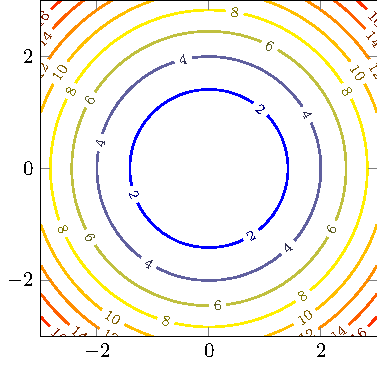
\includegraphics{figures/level_sets.pdf}
    \caption{Level Sets of $f(x, y) = x^2 + y^2$}\label{fig:level_sets}
\end{figure}

\section{Limit and Continuity}

\begin{definition}[Limits]
    The limit of a function of two variables $f(x, y)$ as $(x, y)$ approaches $(x_0, y_0)$ is $L$ and we write 
    \[
        \lim_{(x, y) \to (x_0, y_0)} f(x, y) = L.
    \]
    if for every $\epsilon > 0$, there exists a $\delta > 0$ such that whenever $0 < \| \vec{x} - \vec{x_0} \| < \delta$, it follows that $|f(\vec{x}) - L| < \epsilon$.
\end{definition}

\begin{example}
    Show that the limit below does not exists:
    \[
        \lim_{(x, y) \to (0, 0)} \frac{x^2 - y^2}{x^2 + y^2}.
    \]
\end{example}
\begin{solution}
    Let $f(x, y) = \frac{x^2 - y^2}{x^2 + y^2}$. We will approach the point $(0, 0)$ along two different paths: $x$-axis and $y$-axis.

    \begin{itemize}
        \item Along the $x$-axis ($y = 0$):
        \[
            f(x, 0) = \frac{x^2 - 0^2}{x^2 + 0^2} = \frac{x^2}{x^2} = 1.
        \]
        Thus,
        \[
            \lim_{x \to 0} f(x, 0) = 1.
        \]
        
        \item Along the $y$-axis ($x = 0$):
        \[
            f(0, y) = \frac{0^2 - y^2}{0^2 + y^2} = \frac{-y^2}{y^2} = -1.
        \]
        Thus,
        \[
            \lim_{y \to 0} f(0, y) = -1.
        \]
    \end{itemize}

    Since the limits along the two different paths are not equal (1 and -1), the limit $\lim_{(x, y) \to (0, 0)} f(x, y)$ does not exist.
\end{solution}

\begin{example}
    Does the limit below exist? If it exists, find the limit.
    \[
        \lim_{(x, y) \to (0, 0)} \frac{xy}{x^2 + y^2}.
    \]
\end{example}
\begin{solution}
    Although approaching along the $x$-axis and $y$-axis both give the limit 0, we need to check other paths to confirm the existence of the limit.

    Let's approach the point $(0, 0)$ along the line $y = mx$, where $m$ is a constant. Substituting $y = mx$ into the function, we have:
    \[
        f(x, mx) = \frac{x(mx)}{x^2 + (mx)^2} = \frac{mx^2}{x^2 + m^2x^2} = \frac{mx^2}{x^2(1 + m^2)} = \frac{m}{1 + m^2}.
    \]
    As $x \to 0$, the expression $\frac{m}{1 + m^2}$ remains constant and depends on the value of $m$. Since the limit depends on the slope $m$ of the line we choose to approach $(0, 0)$, the limit does not exist.
\end{solution}

\begin{example}
    Find the limit below, if it exists:
    \[
        \lim_{(x, y) \to (0, 0)} \frac{3x^2 y}{x^2 + y^2}.
    \]
\end{example}
\begin{solution}
    Let $\epsilon > 0$. We need to find a $\delta > 0$ such that whenever $0 < \sqrt{x^2 + y^2} < \delta$, it follows that
    \[
        \left| \frac{3x^2 y}{x^2 + y^2} - 0 \right| < \epsilon \Leftrightarrow \frac{3x^2 |y|}{x^2 + y^2} < \epsilon.
    \]
    Note that $x^2 \leq x^2 + y^2$, so we have
    \[
        \frac{3x^2 |y|}{x^2 + y^2} \leq 3|y| = 3\sqrt{y^2} \leq 3\sqrt{x^2 + y^2}.
    \]
    Thus, we choose $\delta = \frac{\epsilon}{3}$. Then, whenever $0 < \sqrt{x^2 + y^2} < \delta$, we have
    \[
        \frac{3x^2 |y|}{x^2 + y^2} \leq 3\sqrt{x^2 + y^2} < 3 \cdot \frac{\epsilon}{3} = \epsilon.
    \]
    Therefore, the limit is:
    \[
        \lim_{(x, y) \to (0, 0)} \frac{3x^2 y}{x^2 + y^2} = 0.
    \]
\end{solution}

If we drop the condition that $0 < \| \vec{x} - \vec{x_0} \|$, we get the definition of continuity.

\begin{definition}[Continuity]
    A function $f(x, y)$ is continuous at the point $(x_0, y_0)$ if for every $\epsilon > 0$, there exists a $\delta > 0$ such that whenever $\| \vec{x} - \vec{x_0} \| < \delta$, it follows that $|f(\vec{x}) - f(\vec{x_0})| < \epsilon$.
\end{definition}

Note that any polynomial function of several variables is continuous everywhere in its domain.

\section{Partial Derivatives}

\begin{definition}[Partial Derivatives]
    The partial derivative of a function $f(x, y)$ with respect to $x$ at the point $(x_0, y_0)$ is defined as:
    \[
        f_x(x_0, y_0) = \lim_{h \to 0} \frac{f(x_0 + h, y_0) - f(x_0, y_0)}{h}
    \]
    Similarly, the partial derivative of $f(x, y)$ with respect to $y$ at the point $(x_0, y_0)$ is defined as:
    \[
        f_y(x_0, y_0) = \lim_{h \to 0} \frac{f(x_0, y_0 + h) - f(x_0, y_0)}{h}
    \]
\end{definition}

If we let $(x_0, y_0)$ be any point in the domain of $f(x, y)$, then the partial derivatives $f_x(x_0, y_0)$ and $f_y(x_0, y_0)$ represent the rates of change of the function $f(x, y)$ in the $x$ and $y$ directions, respectively, at that point. We have the following notations for partial derivatives:
\[
    f_x = \dfrac{\partial f}{\partial x} = \partial_x f = D_x f, \quad f_y = \dfrac{\partial f}{\partial y} = \partial_y f = D_y f.
\]

For higher order partial derivatives, we can interchange the order of differentiation if the function is sufficiently smooth (i.e., the mixed partial derivatives are continuous). This is known as Clairaut's theorem or Schwarz's theorem:
\[
    f_{xy} = f_{yx}
\]

\section{Tangent Planes and Linear Approximations}

Given a function of two variables $z = f(x, y)$, the tangent plane to the surface at the point $(x_0, y_0, z_0)$ is given by:
\[
    z - z_0 = f_x(x_0, y_0)(x - x_0) + f_y(x_0, y_0)(y - y_0)
\]

If $z = f(x, y)$, then $f$ is differentiable at $(x_0, y_0)$ if the linear approximation:
\[
    L(x, y) = f(x_0, y_0) + f_x(x_0, y_0)(x - x_0) + f_y(x_0, y_0)(y - y_0)
\]
approximates $f(x, y)$ well near the point $(x_0, y_0)$. In other words, the function $f(x, y)$ can be approximated by its tangent plane near the point $(x_0, y_0)$.

Differential of $f$:
\[
    df = f_x(x, y) dx + f_y(x, y) dy
\]

\section{The Chain Rule}

Suppose $z = f(x, y)$, where $x = g(t)$ and $y = h(t)$ are functions of $t$. Then the derivative of $z$ with respect to $t$ is given by:
\[
    \frac{dz}{dt} = \frac{\partial f}{\partial x} \frac{dx}{dt} + \frac{\partial f}{\partial y} \frac{dy}{dt}
\]

\section{Directional Derivatives and Gradient Vectors}

\begin{definition}[Gradient Vector]
    The gradient vector of a function $f(x, y)$ is defined as:
    \[
        \nabla f(x, y) = \left\langle \frac{\partial f}{\partial x}, \frac{\partial f}{\partial y} \right\rangle = \langle f_x, f_y \rangle
    \]
\end{definition}

\begin{definition}[Directional Derivatives]
    The directional derivative of a function $f(x, y)$ at the point $(x_0, y_0)$ in the direction of a unit vector $\mathbf{u} = \langle u_1, u_2 \rangle$ is defined as:
    \[
        D_{\mathbf{u}} f(x_0, y_0) = \lim_{h \to 0} \frac{f(x_0 + hu_1, y_0 + hu_2) - f(x_0, y_0)}{h}
    \]
    Alternatively, it can be computed using the gradient vector:
    \[
        D_{\mathbf{u}} f(x_0, y_0) = \nabla f(x_0, y_0) \cdot \mathbf{u} = f_x(x_0, y_0) u_1 + f_y(x_0, y_0) u_2
    \]
\end{definition}

\section{Maximum and Minimum Values}

We first find the critical points of the function by solving the system of equations:
\[
    f_x(x, y) = 0, \quad f_y(x, y) = 0.
\]

Next, we use the second derivative test to classify the critical points. We compute the second partial derivatives:
\[
    D = \begin{vmatrix}
        f_{xx} & f_{xy} \\
        f_{yx} & f_{yy}
    \end{vmatrix}
    = f_{xx} f_{yy} - (f_{xy})^2.
\]
We have the following cases:
\begin{itemize}
    \item If $D > 0$ and $f_{xx} > 0$, then $f$ has a local minimum at the critical point.
    \item If $D > 0$ and $f_{xx} < 0$, then $f$ has a local maximum at the critical point.
    \item If $D < 0$, then $f$ has a saddle point at the critical point.
    \item If $D = 0$, the test is inconclusive.
\end{itemize}

\section{Lagrange Multipliers}

To find the extrema of a function $f(x, y)$ subject to a constraint $g(x, y) = c$, we introduce a Lagrange multiplier $\lambda$ and solve the system of equations:
\[
    \nabla f(x, y) = \lambda \nabla g(x, y), \quad g(x, y) = c.
\]

If we have more than one constraint, say $g_1(x, y, z) = c_1$ and $g_2(x, y, z) = c_2$, we introduce two Lagrange multipliers $\lambda_1$ and $\lambda_2$ and solve the system of equations:
\[
    \nabla f(x, y, z) = \lambda_1 \nabla g_1(x, y, z) + \lambda_2 \nabla g_2(x, y, z), \quad g_1(x, y, z) = c_1, \quad g_2(x, y, z) = c_2.
\]


\chapter{Multiple Integrals}
\section{Partial Integration}
    We have learnt how to calculate the integration of a function in single variable. Now, we extends our knowledge to functions in several variables. One should understand that the partial integration is the reverse process of partial differentiation.
    \\\indent Define a function $f(x,y):\R^2\to\R$, we have 
    \[\int f dx \quad \text{and}\quad \int f dy\]
    Note that the above integrals are not the same as the single variable integration since $f$ is a function of two variables. The above integrals are called \textbf{partial integrals}. In general, we have 
    \\Given a function $f:\R^n \to \R$
    \[\int f dx_1,\quad \int f dx_2,\quad \dots ,\quad \int f dx_n\]
    where $x_1,x_2,\ldots,x_n$ are the variables of integration.
    \begin{example}
        Given a function $f(x,y)=x^2y+3xy^2$, find $\int f dx$ and $\int f dy$.
        \begin{solution}
            Notice that when we integrate with respect to $x$, we treat $y$ as a constant. So as the other way around. Thus, 
            \[
            \begin{split}
                \int x^2y+3xy^2 dx&= \frac{y}{3}x^3+\frac{3y^2}{2}x^2 +C(y)\\
                \int x^2y+3xy^2 dy&= \frac{x^2}{2}y^2+xy^3 +C(x)
            \end{split}
            \]
        \end{solution}
        The integration constants $C(y)$ and $C(x)$ in this case are functions in $x$ and $y$ rather than just a constant number.
    \end{example}

    \begin{example}
        Given $f(x,y)=ye^{xy^2}$, find $\int f dx$ and $\int f dy$.
        \begin{solution}
            \[
            \begin{split}
                \int ye^{xy^2} dx&= \frac{e^{xy^2}}{y}+C(y)\\
                \int ye^{xy^2} dy&= \frac{1}{2x}e^{xy^2}+C(x)
            \end{split}
            \]
            We can substitute $u=xy^2$, then $du=y^2dx$ and $du=2xy dy$ to compute the integrals.
        \end{solution}
    \end{example}

    \section{Definite integration}
    The concept here is similar to the single variable definite integration. We define the definite partial integral of $f(x,y)$ with respect to $x$ from $a$ to $b$ as
    \[\int_a^b f(x,y) dx =\int_{x=a}^{x=b} f(x,y) dx= F(b,y)-F(a,y)\]
    Similarly, we may define the definite partial integral of $f(x,y)$ with respect to $y$ from $c$ to $d$ as
    \[\int_c^d f(x,y) dy =\int_{y=c}^{y=d} f(x,y) dy= G(x,d)-G(x,c)\]
    Note that $y$ and $x$ are treated as constants in the above two definitions respectively.

    \begin{example}
        Given $f(x,y)=x^2y+3xy^2$, find $\int_1^3 f(x,y) dx$ and $\int_1^3 f(x,y) dy$.
        \begin{solution}
            \[
            \begin{split}
                \int_1^3 (x^2y+3xy^2) dx&= \left[\frac{y}{3}x^3+\frac{3y^2}{2}x^2\right]_{x=1}^{x=3}= \frac{26}{3}y + 12y^2\\
                \int_1^3 (x^2y+3xy^2) dy&= \left[\frac{x^2}{2}y^2+xy^3\right]_{y=1}^{y=3}= 4x^2 + 26x
            \end{split}
            \]
        \end{solution}
    \end{example}

    \section{Double Integrals}
    A double integral is an extension of the single variable definite integral to functions of two variables. It is used to calculate the volume under a surface defined by a function $f(x,y)$ over a rectangular region in the $xy$-plane. The double integral of $f(x,y)$ over the rectangular region $R = [a,b] \times [c,d]$ is denoted as:
    \[\iint_R f(x,y) dA = \int_a^b \int_c^d f(x,y) dy dx\]
    where $dA$ represents a small area element on the $xy$-plane.



\chapter{Vector Calculus}

\end{document}